\documentclass[../TakeYourPill.tex]{subfiles}
\graphicspath{{\subfix{images/}}}

\begin{document}

\newpage

\begin{figure}[ht]
  \vfill
  \hfill
  \begin{subfigure}[b]{.3\textwidth}
    \centering
    
\includegraphics[width=\textwidth]{app-intro-screenshot}
    \caption{Úvodní obrazovka}
    \label{fig:intro}
  \end{subfigure}
  \hfill
  \begin{subfigure}[b]{.3\textwidth}
    \centering
    
\includegraphics[width=\textwidth]{homescreen-screenshot}
    \caption{Domovská obrazovka}
    \label{fig:homescreen}
  \end{subfigure}
  \hfill
  \begin{subfigure}[b]{.3\textwidth}
    \centering
    
\includegraphics[width=\textwidth]{pill-details}
    \caption{Detail léku}
    \label{fig:details}
  \end{subfigure}
  \hfill
  \vfill
  \vspace{6pt}
  \hfill
  \begin{subfigure}[b]{.3\textwidth}
    \centering
    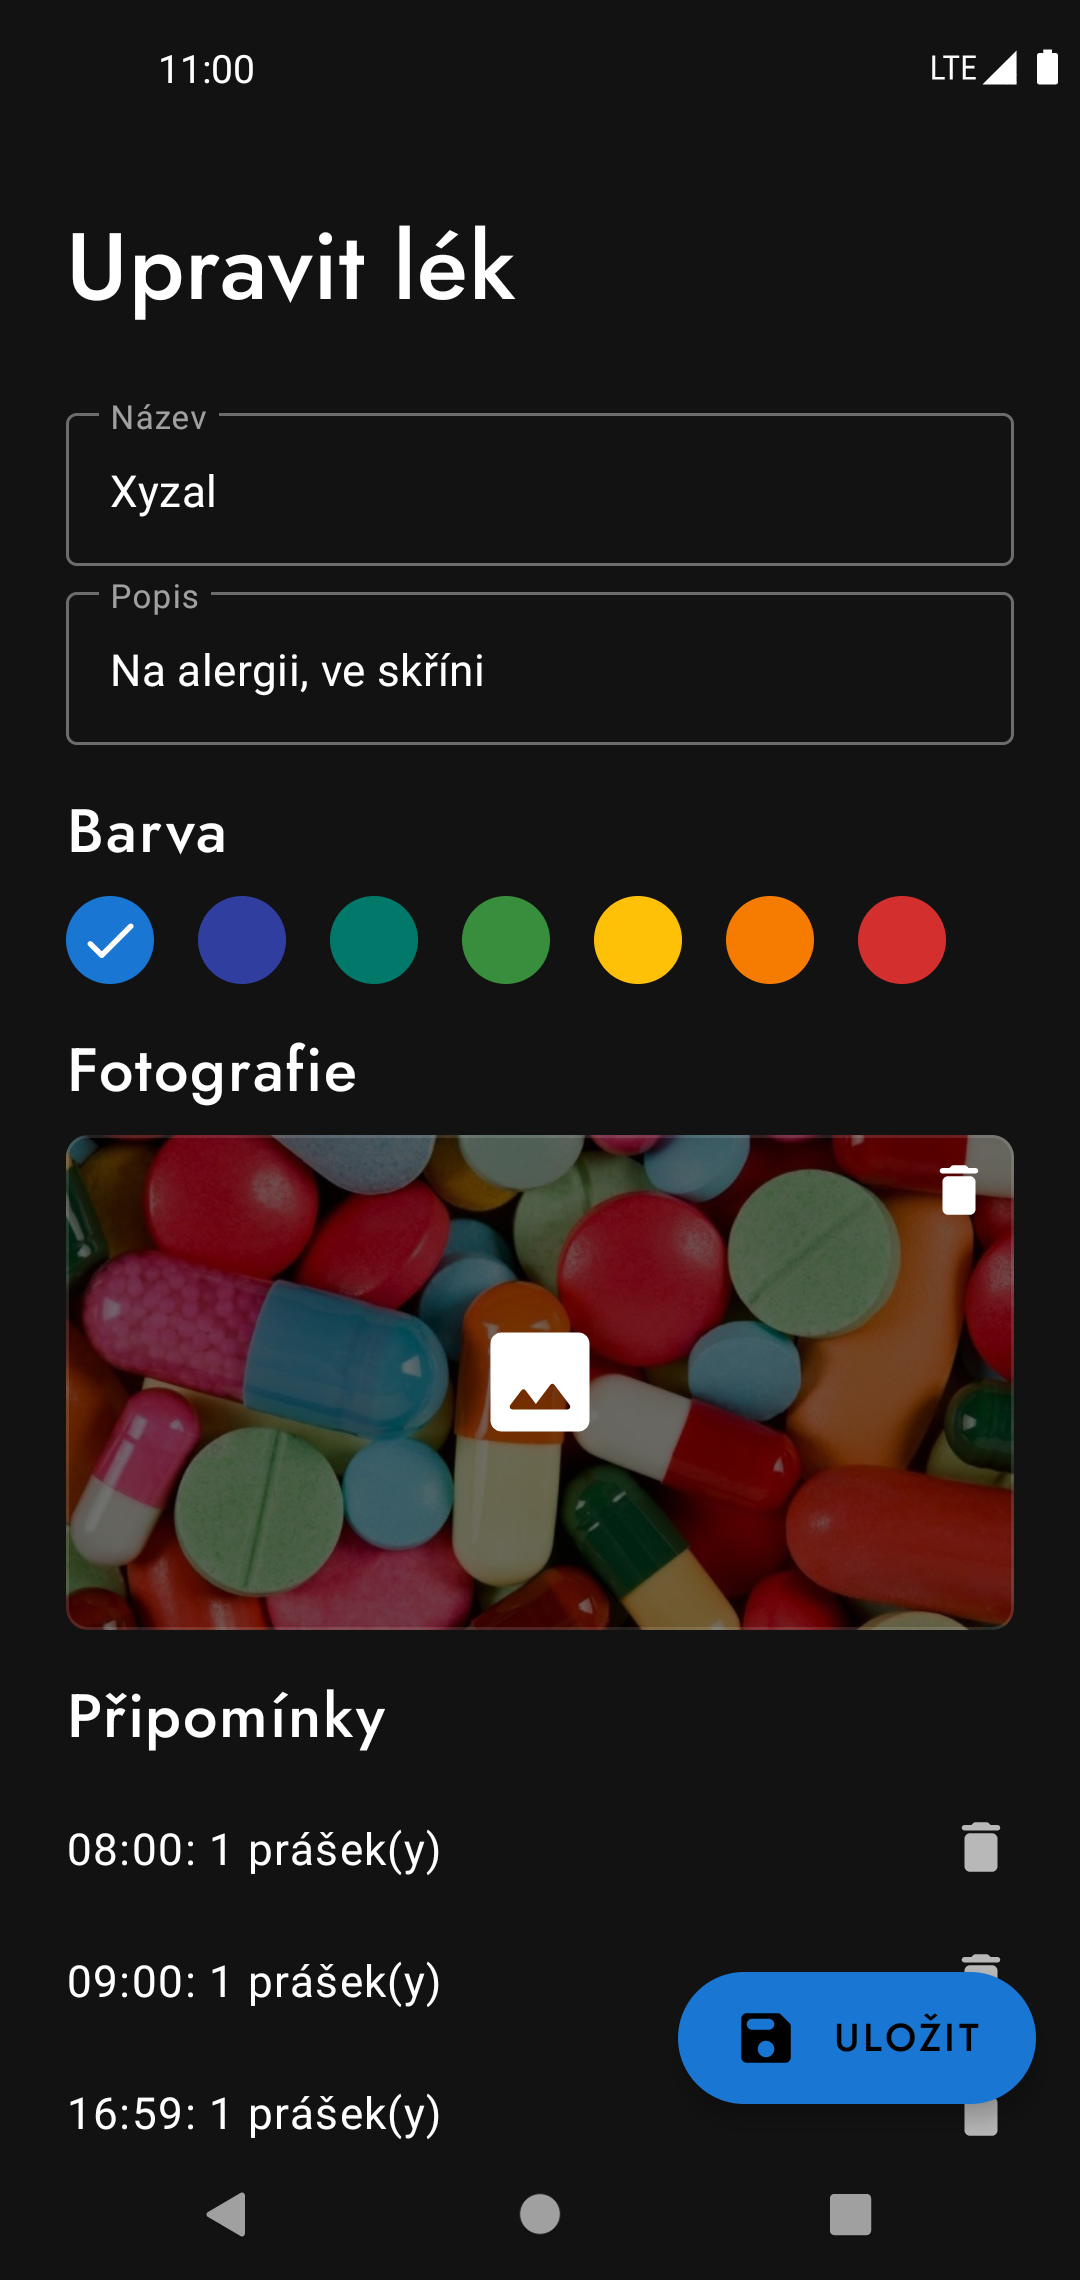
\includegraphics[width=\textwidth]{pill-edit}
    \caption{Úprava léku}
    \label{fig:edit}
  \end{subfigure}
  \hfill
  \begin{subfigure}[b]{.3\textwidth}
    \centering
    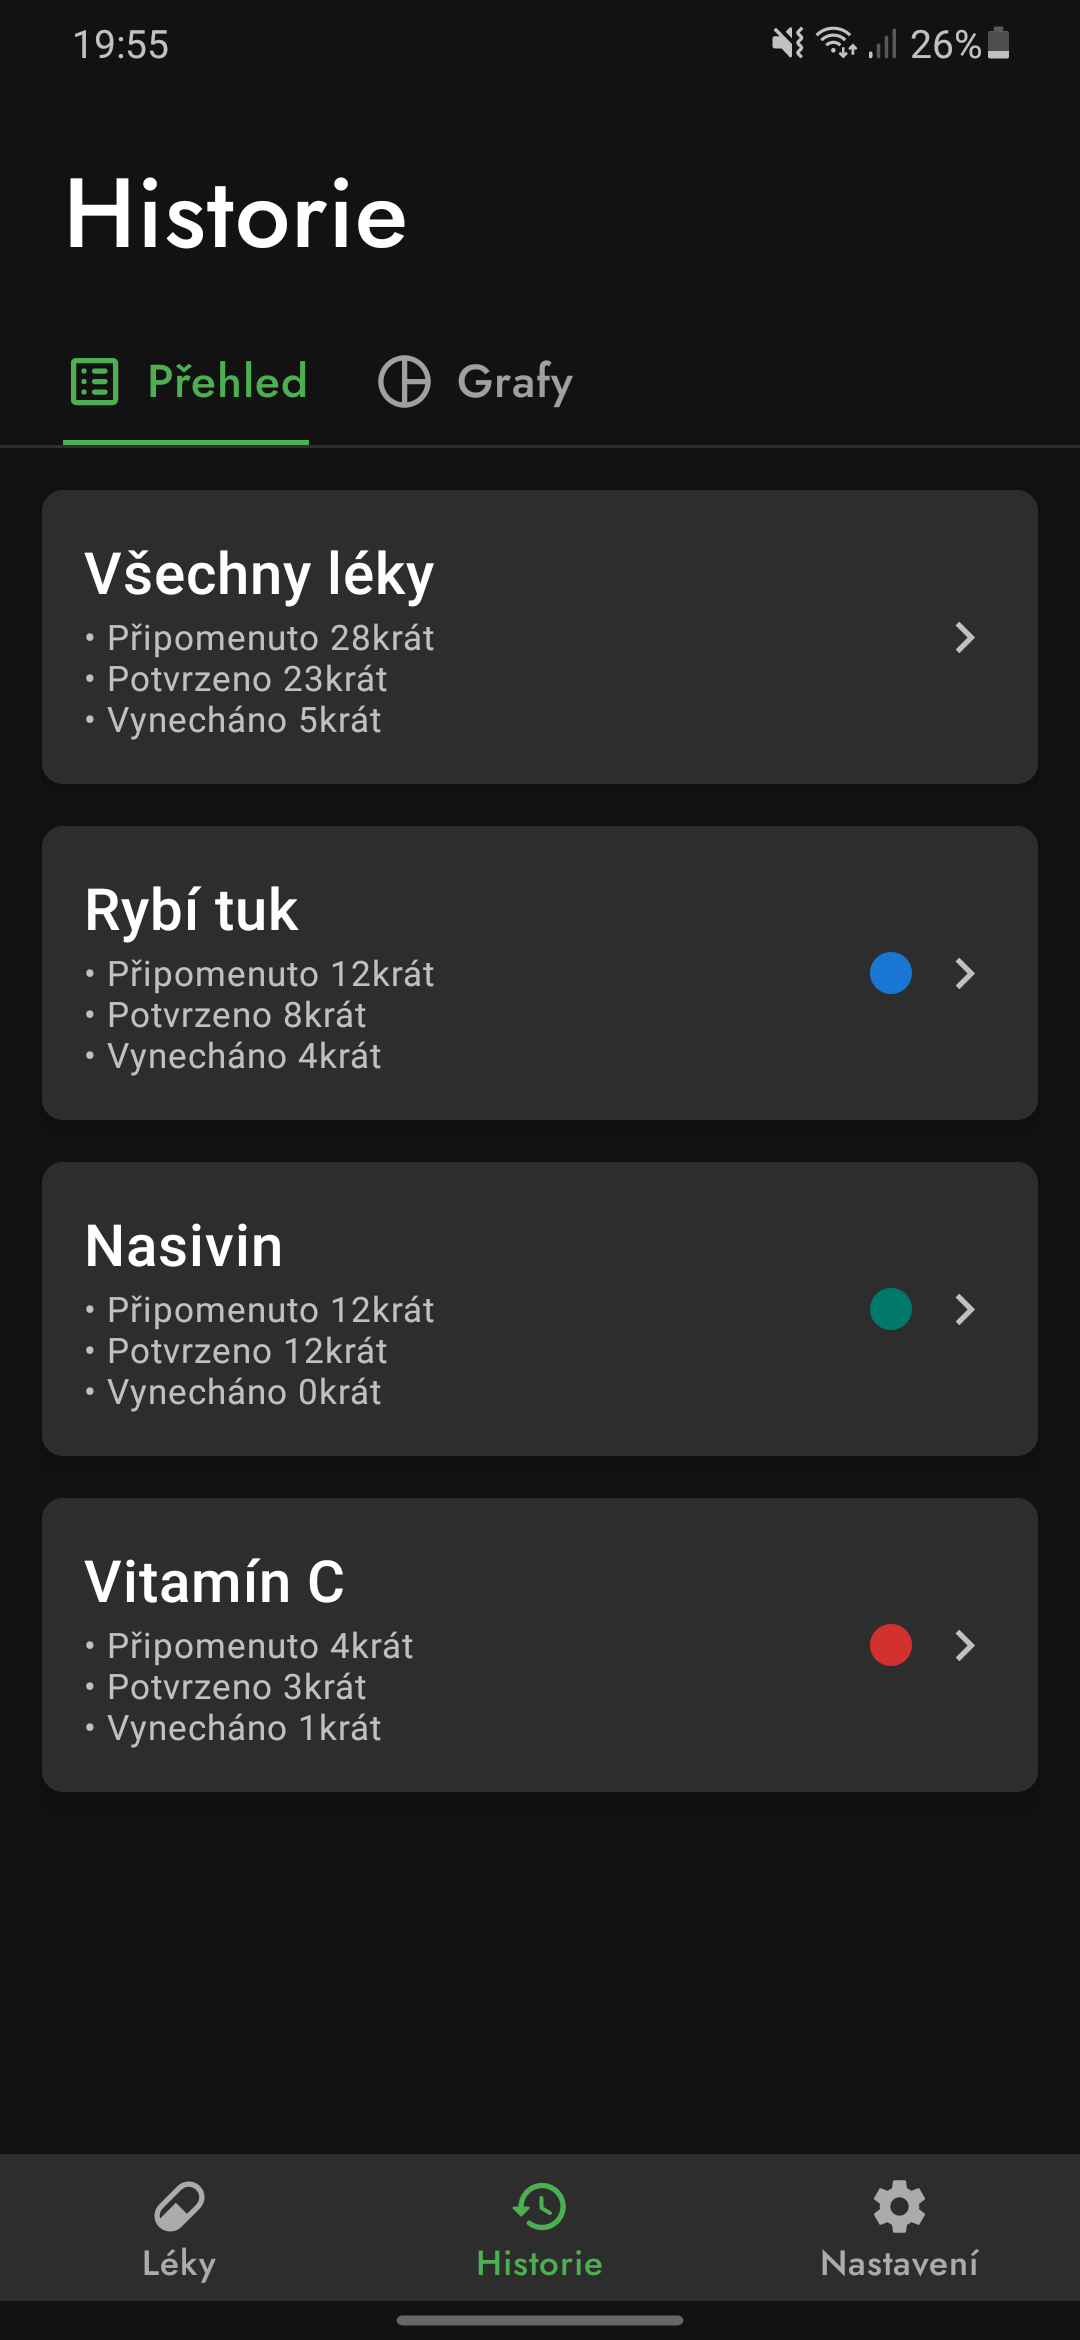
\includegraphics[width=\textwidth]{history-overall}
    \caption{Přehled historie}
    \label{fig:history}
  \end{subfigure}
  \hfill
  \begin{subfigure}[b]{.3\textwidth}
    \centering
    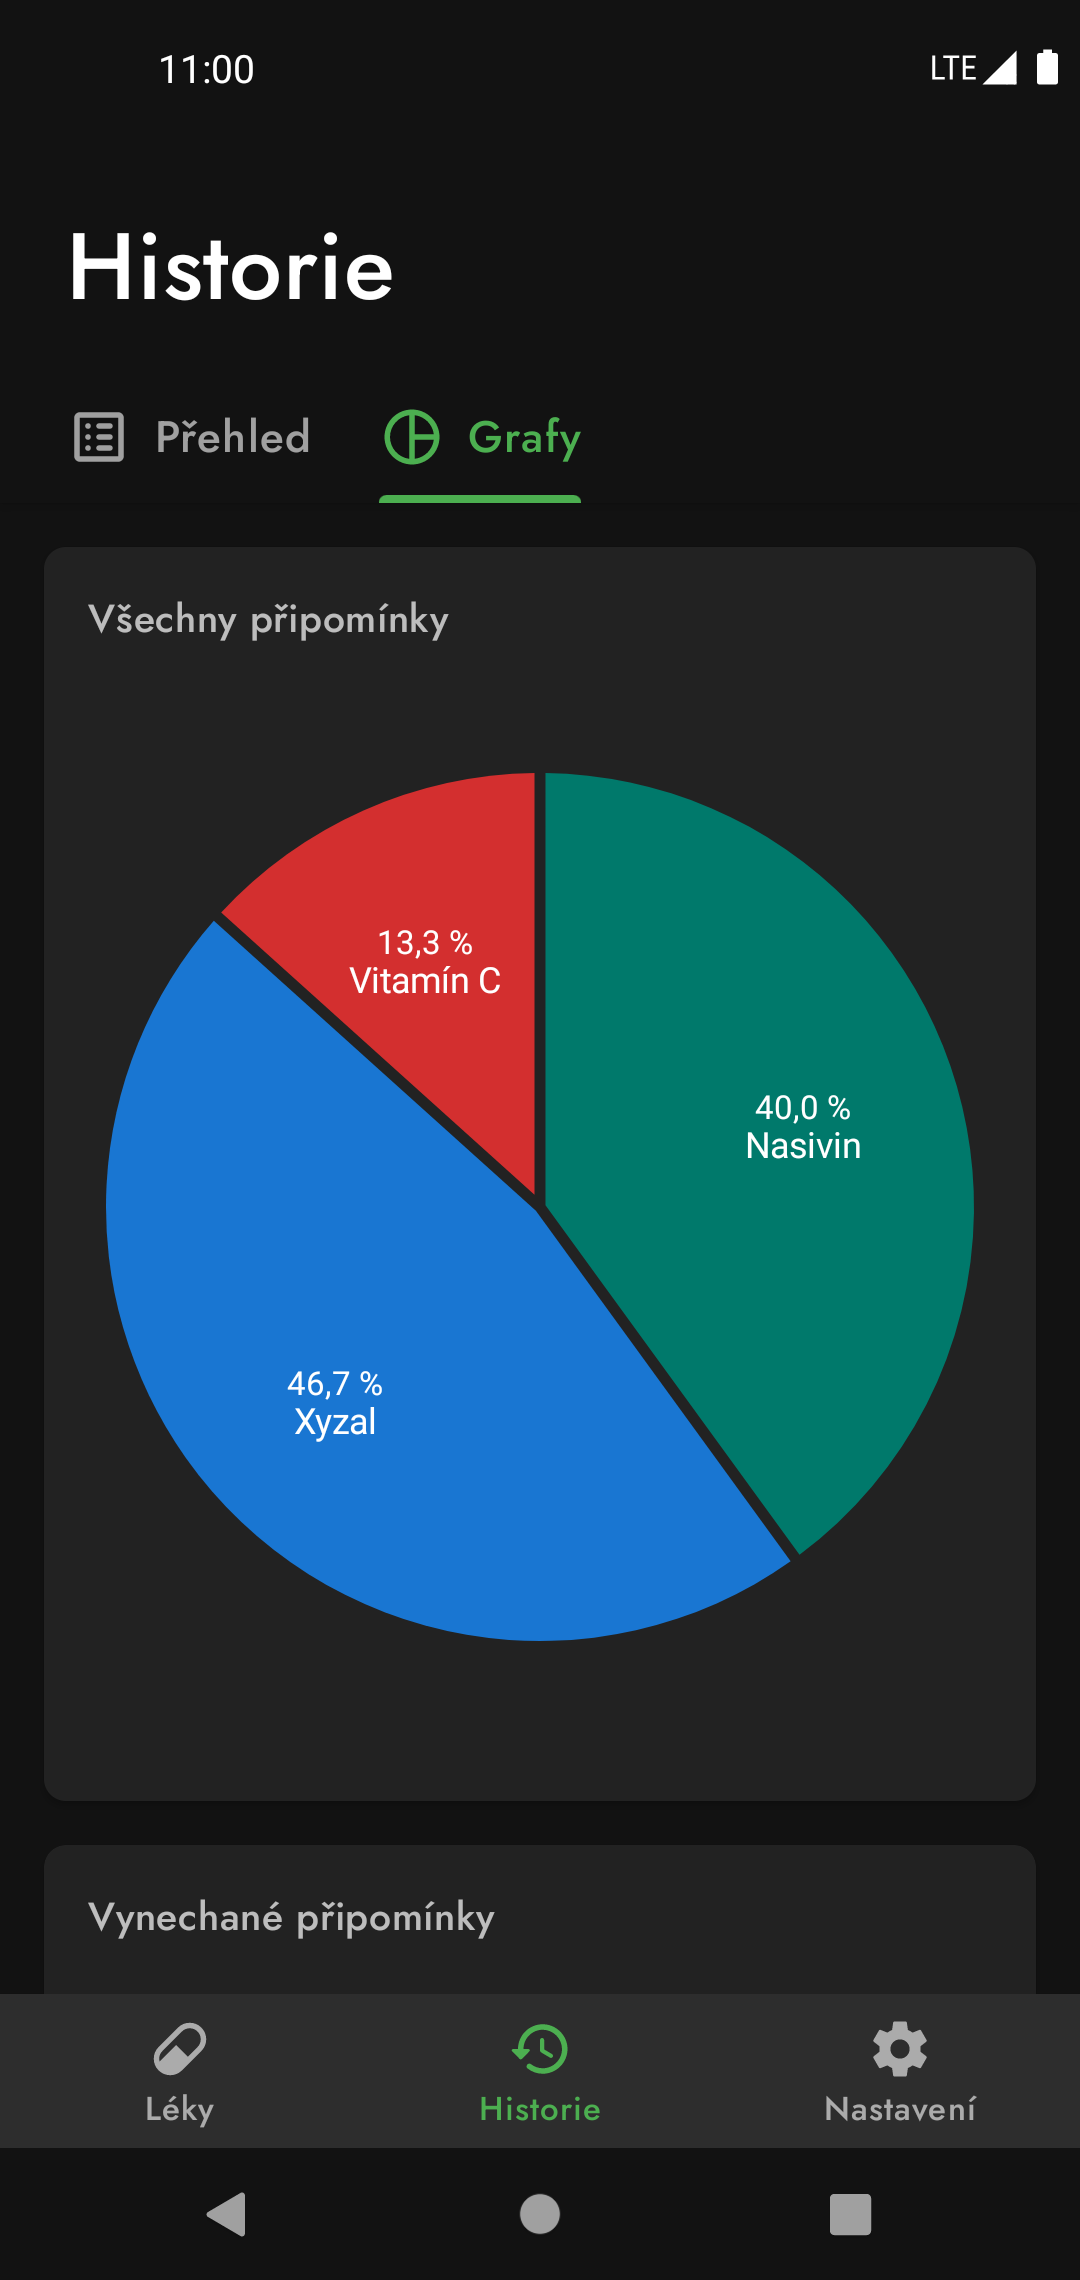
\includegraphics[width=\textwidth]{history-graphs}
    \caption{Grafy}
    \label{fig:graphs}
  \end{subfigure}
  \hfill
  \vfill
\caption{Snímky obrazovky z  aplikace}
\label{fig:screenshots}
\end{figure}

\end{document}
